\section{SectorQ Design}
\label{sec:design}
\SectorQ addresses the locality and capacity limits with three mechanisms.
Window-conserved parity sectors assign equal-string contributions to the same sector throughout a group of gates.
Runtime re-sectoring selects the next partition from window generators and sampled live terms during execution.
Host-memory sector execution separates the stored expansion from the working set of each GPU and redistributes terms at window boundaries.

\subsection{Overall Architecture}
Figure~\ref{fig:overview} shows the circuit processing and the execution loop on each node.
The CPU constructs windows and selects their rows, host memory holds the sectors, and each GPU processes one sector at a time.

\noindent\textbf{Window Formation.}
The \emph{Window Builder} first expresses the circuit in the processing order of the observable.
A Clifford frame absorbs eligible Clifford gates and transforms the generators of subsequent rotations, preserving the action on the observable.
For example, a Hadamard maps the generator $Z_3$ to $X_3$ in the illustrated circuit.
For each window, the builder accumulates the span of the branching generators over $\mathrm{GF}(2)$ and stops before its dimension exceeds the number of qubits.
This bound ensures at least as many independent conserved rows as qubits for run-time partition selection.
The default boundary moves to the last scheduled truncation in the second half of the window when one is available, reducing the terms that require redistribution.
Clifford operations that remain explicit transform generators into a common coordinate system for this calculation.
The resulting window defines a sequence of operations and a space of valid partitions, with the particular rows selected during execution.

\noindent\textbf{Window Loop.}
Each node follows the numbered steps in Figure~\ref{fig:overview}.
At step (1), a GPU worker loads one sector from the \emph{Sector Store} in host memory.
At step (2), its \emph{Sector Executor} applies the current window, including the merges and scheduled truncations.
During these operations, \emph{Runtime Re-Sectoring} uses the CPU to select the rows of the next window.
At step (3), the worker uses these rows to partition its output on the GPU.
Step (4) appends output chunks to the host lists of the next sectors.
The \emph{Sector Exchanger} transfers the remote lists at step (5), assigning sector $d$ to node $d\bmod N$ among $N$ nodes.
Each node then processes its received sectors with the same loop.
The last window evaluates the observable against the input state and reduces the partial answers across nodes.
Each sector is complete before its next window begins, permitting the window's merges and truncations to execute locally.

\begin{figure}[t]
\centering
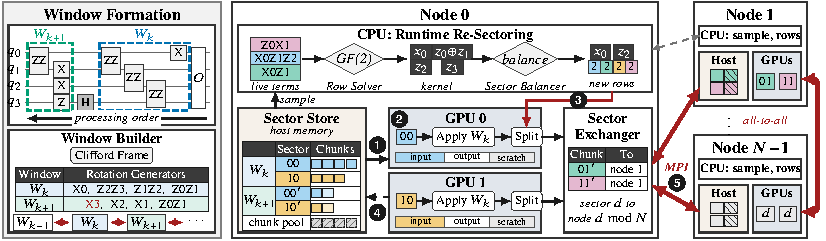
\includegraphics[width=\textwidth]{figures/overview.pdf}
\caption{Overall architecture of \SectorQ}
\label{fig:overview}
\end{figure}

\subsection{Window-Conserved Parity Sectors}
The execution loop requires a partition that preserves merge locality through every operation of a window.
Figure~\ref{fig:sectors} illustrates this condition on four qubits and two parity rows.

\noindent\textbf{Rows Conserved by a Window.}
A Pauli string has a binary representation $v=(x,z)\in\mathrm{GF}(2)^{2n}$, with its phase represented in the coefficient.
For a row $r$, the parity is the binary inner product $r\cdot v$.
A rotation with generator $q$ branches an anticommuting input string $v$ into $v$ and $v\oplus q$.
Their parities agree whenever $r\cdot q=0$.
The \emph{Row Solver} computes the annihilator of the generator span with Gaussian elimination over $\mathrm{GF}(2)$.
If that span has dimension $d$, its annihilator has dimension $2n-d$, at least $n$ under the window rule.
The selected rows form a matrix $R$, and the bit vector $Rv$ labels the sector of $v$.
This binary linear algebra is related to symmetry detection for qubit tapering~\cite{bravyi2017tapering}.
The rows label terms of the observable during one window, retaining the full qubit representation for subsequent windows.

\noindent\textbf{Merge Locality.}
Every descendant of a term retains its sector label through the branching rotations of the window.
This property follows by induction from $R(v\oplus q)=Rv$ for each generator in the window.
A coefficient change from a Pauli noise channel also preserves the string and its label.
For an explicit Clifford operation, the row coordinates transform with the strings to preserve the same label.
Equal strings have equal labels, placing all contributions to a string in one sector before truncation.
Consequently, a merge and coefficient truncation within each complete sector produce the same operator as a global merge and truncation at the same operations, apart from floating-point summation order.
In the example, the rows $x_1$ and $z_0\oplus z_1\oplus z_2\oplus z_3$ label both $Z_0X_1$ and $Y_0X_1$ as sector $11$.
The descendants retain label $11$ throughout $W_k$, allowing their coefficients to be combined before the scheduled truncation.

\noindent\textbf{Exchange Only at Window Boundaries.}
The next window can contain generators that change the current parity labels.
For example, $X_1$ in $W_{k+1}$ changes the parity $x_1$ used by $W_k$.
The runtime computes a new matrix for $W_{k+1}$ and regroups the output of $W_k$ before that window begins.
This regrouping collects all fragments of each next sector on its owner for merging before the next truncation.
The construction differs from a fixed linear partition~\cite{paulistrings}, whose rows can require a remote transfer at a gate that changes a partition label.
It also differs from a partition based only on symmetries of the full circuit, since these symmetries need not distinguish the live terms.
The window rule requires conservation only over the operations assigned to the current sector execution.
The resulting partitions can change at window boundaries while preserving the prescribed truncation schedule.

\begin{figure}[t]
\centering
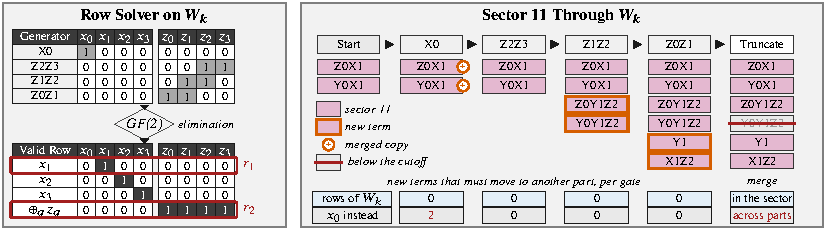
\includegraphics[width=\textwidth]{figures/sectors.pdf}
\caption{Window-conserved parity sectors}
\label{fig:sectors}
\end{figure}

\subsection{Runtime Re-Sectoring}
Conservation determines which rows are valid, but the live terms determine their load balance.
Figure~\ref{fig:resector} shows how the runtime selects the next rows while the GPUs process the current window.

\noindent\textbf{Sampling the Live Terms.}
At the start of a window, each node samples strings from its host sectors with a regular stride determined by the global term count.
The configured sample target is 200,000 terms across all nodes.
The CPU applies the current window's bit-changing Clifford operations to these strings before the next partition is scored.
This estimate applies coordinate changes without reproducing the branching and truncation of the sampled operator.
The sample approximates the string coordinates at the next boundary, with no exact prediction of the output population.
An MPI gather collects the samples on rank zero, where the row solver and the \emph{Sector Balancer} make a common decision for every node.
A broadcast distributes the selected rows and window description.
All workers use the broadcast matrix to assign identical labels to identical strings.
The sample affects performance decisions only, since every selected row must satisfy the generator constraints independently of the sampled terms.

\noindent\textbf{Balanced Row Selection.}
The sector balancer generates eight candidate row sets from random combinations of the annihilator basis.
For each candidate, it counts sampled strings per sector and selects the row set that minimizes the maximum count.
The illustrated pairs produce largest counts of eight, four, and two, and the selected pair $(x_0,z_2)$ divides the eight strings equally.
The number of rows depends on the estimated output size, the target terms per sector, and the available GPUs.
The estimate uses the previous window's observed growth with a bounded growth factor.
The runtime requests one task per GPU, or two when the preceding window exceeds the configured duration threshold, provided the resulting sectors remain sufficiently large.
Windows with few terms use fewer sectors to avoid small GPU tasks.
A configurable cap bounds the number of sectors at a boundary.
Candidate scoring controls the sampled maximum sector size, while the row count controls execution granularity and the number of available tasks.

\noindent\textbf{Overlap with the Running Window.}
The host sample is captured before the workers consume their input sectors.
After the workers start, the CPU main thread gathers the sample, computes the next window, scores the candidate rows, and broadcasts the result.
Workers need those rows only when they partition their output for the next window.
A worker that reaches this point before the rows are ready waits on a local condition variable.
The implementation records this wait separately from CPU selection time to distinguish overlapped selection from a delay visible to workers.
The overlap depends on the relative durations of row selection and sector execution.
Short windows can expose selection latency, whereas longer windows provide more time for the CPU calculation before output partitioning.
The conservation constraints ensure merge locality in both cases, independent of sample quality and the duration of selection.

\begin{figure}[t]
\centering
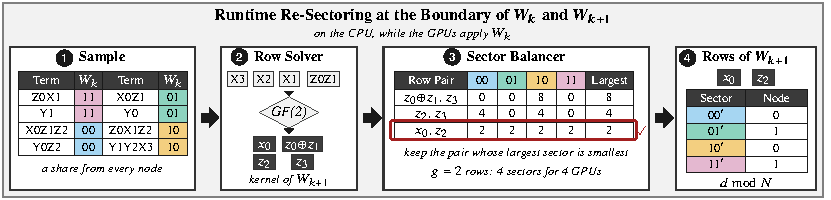
\includegraphics[width=\textwidth]{figures/resector.pdf}
\caption{Runtime re-sectoring at a window boundary}
\label{fig:resector}
\end{figure}

\subsection{Host-Memory Sector Execution and Exchange}
The selected sectors are units of execution rather than permanent GPU allocations.
Figure~\ref{fig:execution} shows their storage, processing, and transfer across a window boundary.

\noindent\textbf{Chunked Sector Store.}
The sector store represents each sector as a list of fixed-capacity host chunks, with 262,144 terms per chunk by default.
Each term contains a binary string and a double-precision coefficient.
A pool retains pinned chunks for reuse after GPU transfers or MPI sends, avoiding repeated registration for every sector.
The same chunk representation supports input loading, output collection, and reception from another node.
A sector can contain multiple chunks, and a node can hold more sectors than it has GPUs.
The live expansion occupies host memory, while only the sectors under execution require GPU buffers.
The total capacity depends on host storage for input, temporary output, and exchanged chunks.
Within a node, workers obtain sectors from a shared queue, initially ordered by decreasing size.
Workers obtain another sector as they finish their current task, redistributing work within the node as sector execution times vary.

\noindent\textbf{Sector Execution on GPUs.}
Each worker maintains input and output expansions together with the library workspace on its GPU.
The worker loads a complete sector, applies its window, and performs the required merges before coefficient truncation.
If the sector is too large to load with sufficient workspace, an additional valid row divides it in host memory.
If growth exhausts the GPU buffers during execution, the worker partitions the current expansion using a further row conserved by the remaining operations.
The resulting subsectors return to the local queue with the operation position and any pending merge or truncation.
Each subsector resumes from that position and preserves merge locality under the finer partition.
A split succeeds only if the available rows distinguish enough terms to fit the working set.
The runtime records host and GPU splits separately.
Host storage can accommodate a larger operator only when its sectors admit subdivisions whose expansions and workspace fit an individual GPU.

\noindent\textbf{Boundary Exchange.}
At the end of a window, a GPU partitions its surviving terms by the next matrix and copies them into host chunks.
Chunks for local sectors remain on the node, and the sector exchanger sends the other chunks to their owners.
The exchange first communicates counts and then transfers the chunks in rounds.
For each sender and destination sector, a round transfers at most one chunk.
After the outstanding requests complete, the sender returns transmitted chunks to the pool before the next round begins.
Additional receive storage is bounded by one round, and the request count depends on active sender-sector pairs.
At completion, the owner joins the received chunk lists into each complete next sector.
A checkpoint can record this boundary state and its next-window description.
Chunk reuse permits output collection and redistribution without allocating a second receive buffer for the entire expansion.

\begin{figure}[t]
\centering
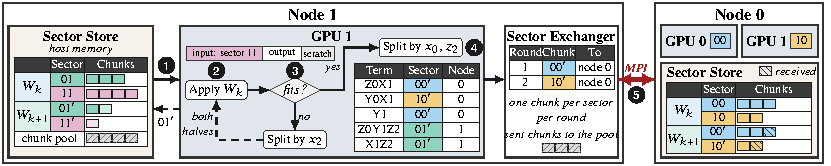
\includegraphics[width=\textwidth]{figures/execution.pdf}
\caption{Host-memory sector execution and boundary exchange with pale filling chunks, black-hatched received chunks, and gray-hatched pooled chunks}
\label{fig:execution}
\end{figure}

\subsection{Implementation}
\SectorQ implements the host runtime in C++ and the string partition operations in CUDA.
Each MPI rank owns one node and creates one worker per GPU, with four GPUs per node in our experiments.

\noindent\textbf{Runtime and Library Operations.}
Each worker uses \cuPP~v0.5.0 on one GPU.
The library operations cover rotations, Clifford gates, Pauli noise, merging, and truncation.
The runtime supplies the sector contents and manages their placement, while the library supplies the arithmetic on each expansion.
CUDA kernels evaluate the row parities and group output terms by their next sectors.
The CPU handles binary elimination, sample scoring, the host chunk pool, and MPI exchange.
Consecutive Pauli noise channels can share a library call up to the next truncation, preserving the scheduled coefficient decisions.
On one GPU, an expansion below the target sector size can remain in device memory between windows.
This path avoids a host transfer when no other worker could receive a sector.
Both optimizations preserve the window partition and its scheduled coefficient decisions.
Table~\ref{tab:parameters} summarizes the default parameters and the larger sector caps used in the capacity experiments.

\begin{table}[t]
\caption{Runtime parameters}
\label{tab:parameters}
\centering
\small
\begin{tabular}{@{}ll@{}}
\toprule
\textbf{Parameter} & \textbf{Setting} \\
\midrule
Sample target across nodes & 200,000 terms \\
Candidate row sets & 8 \\
Target sector input & 4 million terms, 6 million for kicked Ising \\
Tasks per GPU & 1, or 2 after a window of at least 0.5~s \\
Default sector cap & 256 \\
Capacity experiment sector caps & 1,024 or 4,096 \\
Host chunk capacity & 262,144 terms, 65,536 for selected large runs \\
GPU memory budget & 90\% of available device memory \\
Each expansion buffer & 20\% of the GPU memory budget \\
Coefficient truncation & Every 10 operations by default \\
\bottomrule
\end{tabular}
\end{table}
